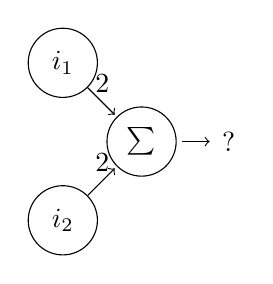
\begin{tikzpicture}[shorten >=1pt,->, node distance=\layersep]
    \tikzstyle{every pin edge}=[<-,shorten <=2pt]
    \tikzstyle{neuron}=[circle,draw,minimum size=25pt,inner sep=0pt]
    \tikzstyle{output neuron}=[draw,minimum size=25pt, minimum width=50pt,inner sep=0pt]
    \tikzstyle{input neuron}=[neuron];
    \tikzstyle{hidden neuron}=[neuron];
    \tikzstyle{annot} = [text centered]

    % Draw the input layer nodes
    \node[input neuron] (I-1) at (0,1) {$i_{1}$};
    \node[input neuron] (I-2) at (0,-1) {$i_{2}$};

    % Draw the hidden layer nodes
    \node[neuron ,pin={[pin edge={->}]right:?}] (H-1) at (\layersep,0) {$\sum$};

    % Connect every node in the input layer with every node in the
    % hidden layer.
    \path (I-1) edge node[above]{2} (H-1);
    \path (I-2) edge node[above]{2} (H-1);

\end{tikzpicture}
